% http://tex.stackexchange.com/questions/11866/compile-a-latex-document-into-a-png-image-thats-as-short-as-possible#11880
%http://tex.stackexchange.com/questions/152247/best-practice-to-include-standalone-precompiled-graphics
\documentclass[border=1pt]{standalone}
\usepackage{tikz}

\begin{document}

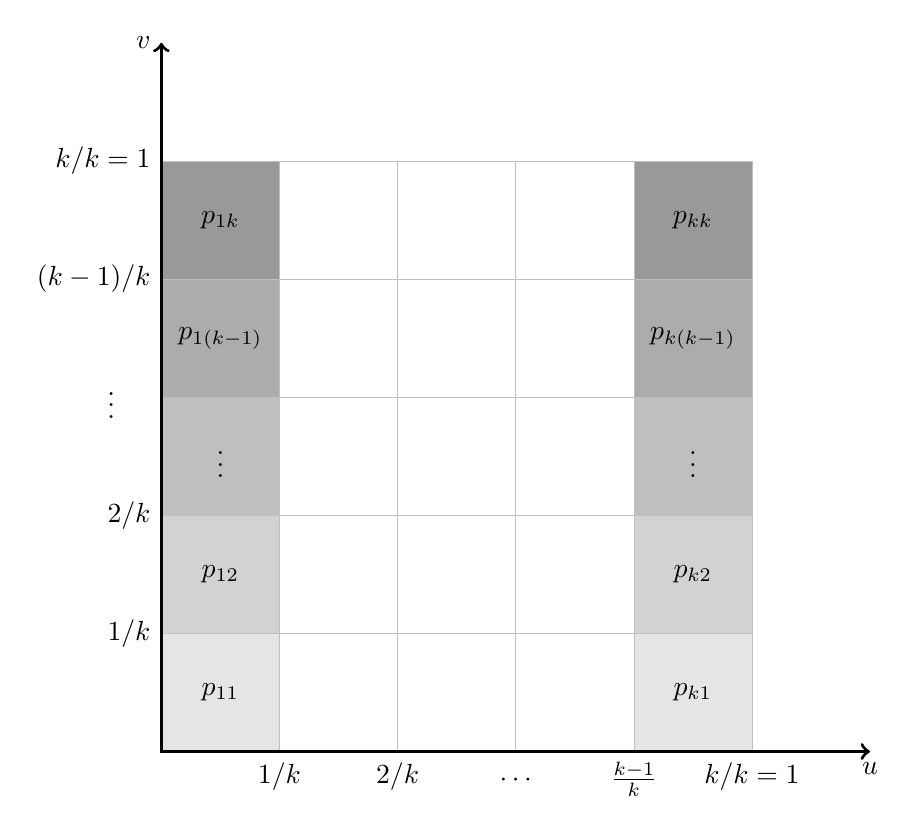
\begin{tikzpicture}[very thick, scale=1.5]

	\fill[color=gray!20] (0, 0) rectangle (1, 0+1);
	\fill[color=gray!35] (0, 1) rectangle (1, 1+1);
	\fill[color=gray!50] (0, 2) rectangle (1, 2+1);
	\fill[color=gray!65] (0, 3) rectangle (1, 3+1);
	\fill[color=gray!80] (0, 4) rectangle (1, 4+1);
	\fill[color=gray!20] (4, 0) rectangle (5, 0+1);
	\fill[color=gray!35] (4, 1) rectangle (5, 1+1);
	\fill[color=gray!50] (4, 2) rectangle (5, 2+1);
	\fill[color=gray!65] (4, 3) rectangle (5, 3+1);
	\fill[color=gray!80] (4, 4) rectangle (5, 4+1);

	\coordinate (A1) at (0,0);
	\coordinate (A2) at (5,5);
	\draw [help lines, lightgray] (A1) grid (A2);
	\draw[<->] (0,6) node[left] {$v$} -- (0,0) -- (6,0) node[below] {$u$};

	\node[left] at (0,1) {$1/k$};
	\node[left] at (0,2) {$2/k$};
	\node[left] at (-0.3,3) {$\vdots$};
	\node[left] at (0,4) {$(k-1)/k$};
	\node[left] at (0,5) {$k/k = 1$};
	
	\node at (0.5,0.5) {$p_{11}$};
	\node at (0.5,1.5) {$p_{12}$};
	\node at (0.5,2.5) {$\vdots$};
	\node at (0.5,3.5) {$p_{1(k-1)}$};
	\node at (0.5,4.5) {$p_{1k}$};

	\node at (4.5,0.5) {$p_{k1}$};
	\node at (4.5,1.5) {$p_{k2}$};
	\node at (4.5,2.5) {$\vdots$};
	\node at (4.5,3.5) {$p_{k(k-1)}$};
	\node at (4.5,4.5) {$p_{kk}$};

	\node[below] at (1,0) {$1/k$};
	\node[below] at (2,0) {$2/k$};
	\node[below] at (3,-0.1) {$\cdots$};
	\node[below] at (4,0) {$\frac{k-1}{k}$};
	\node[below] at (5,0) {$k/k = 1$};
	


\end{tikzpicture}

\end{document}
